\section{Final Design}

LARRE's leg segments are constructed from 6061 aluminum alloy concentric sliding pipes with clamps allowing the joints' to be adjusted for each person. This material is lightweight and easy to manufacture. The axles of the joints were constructed of steel to handle the expected stress. Safety is a significant concern; careful attention was given to the manufacturing process to minimize the sharp edges since it is attached to a human-machine interface system. Safety is essential for people with SCI who have minimal sensory abilities and would not feel an injury.  LARRE is attached to a person through the upper body and waist straps. Custom-made 3D printed strap carriages are places on the thigh and shank segment. These carriages connect the person to the legs of the exoskeleton. \autoref{fig:LARRE} shows the final model of LARRE.     


\begin{figure}
    \centering
    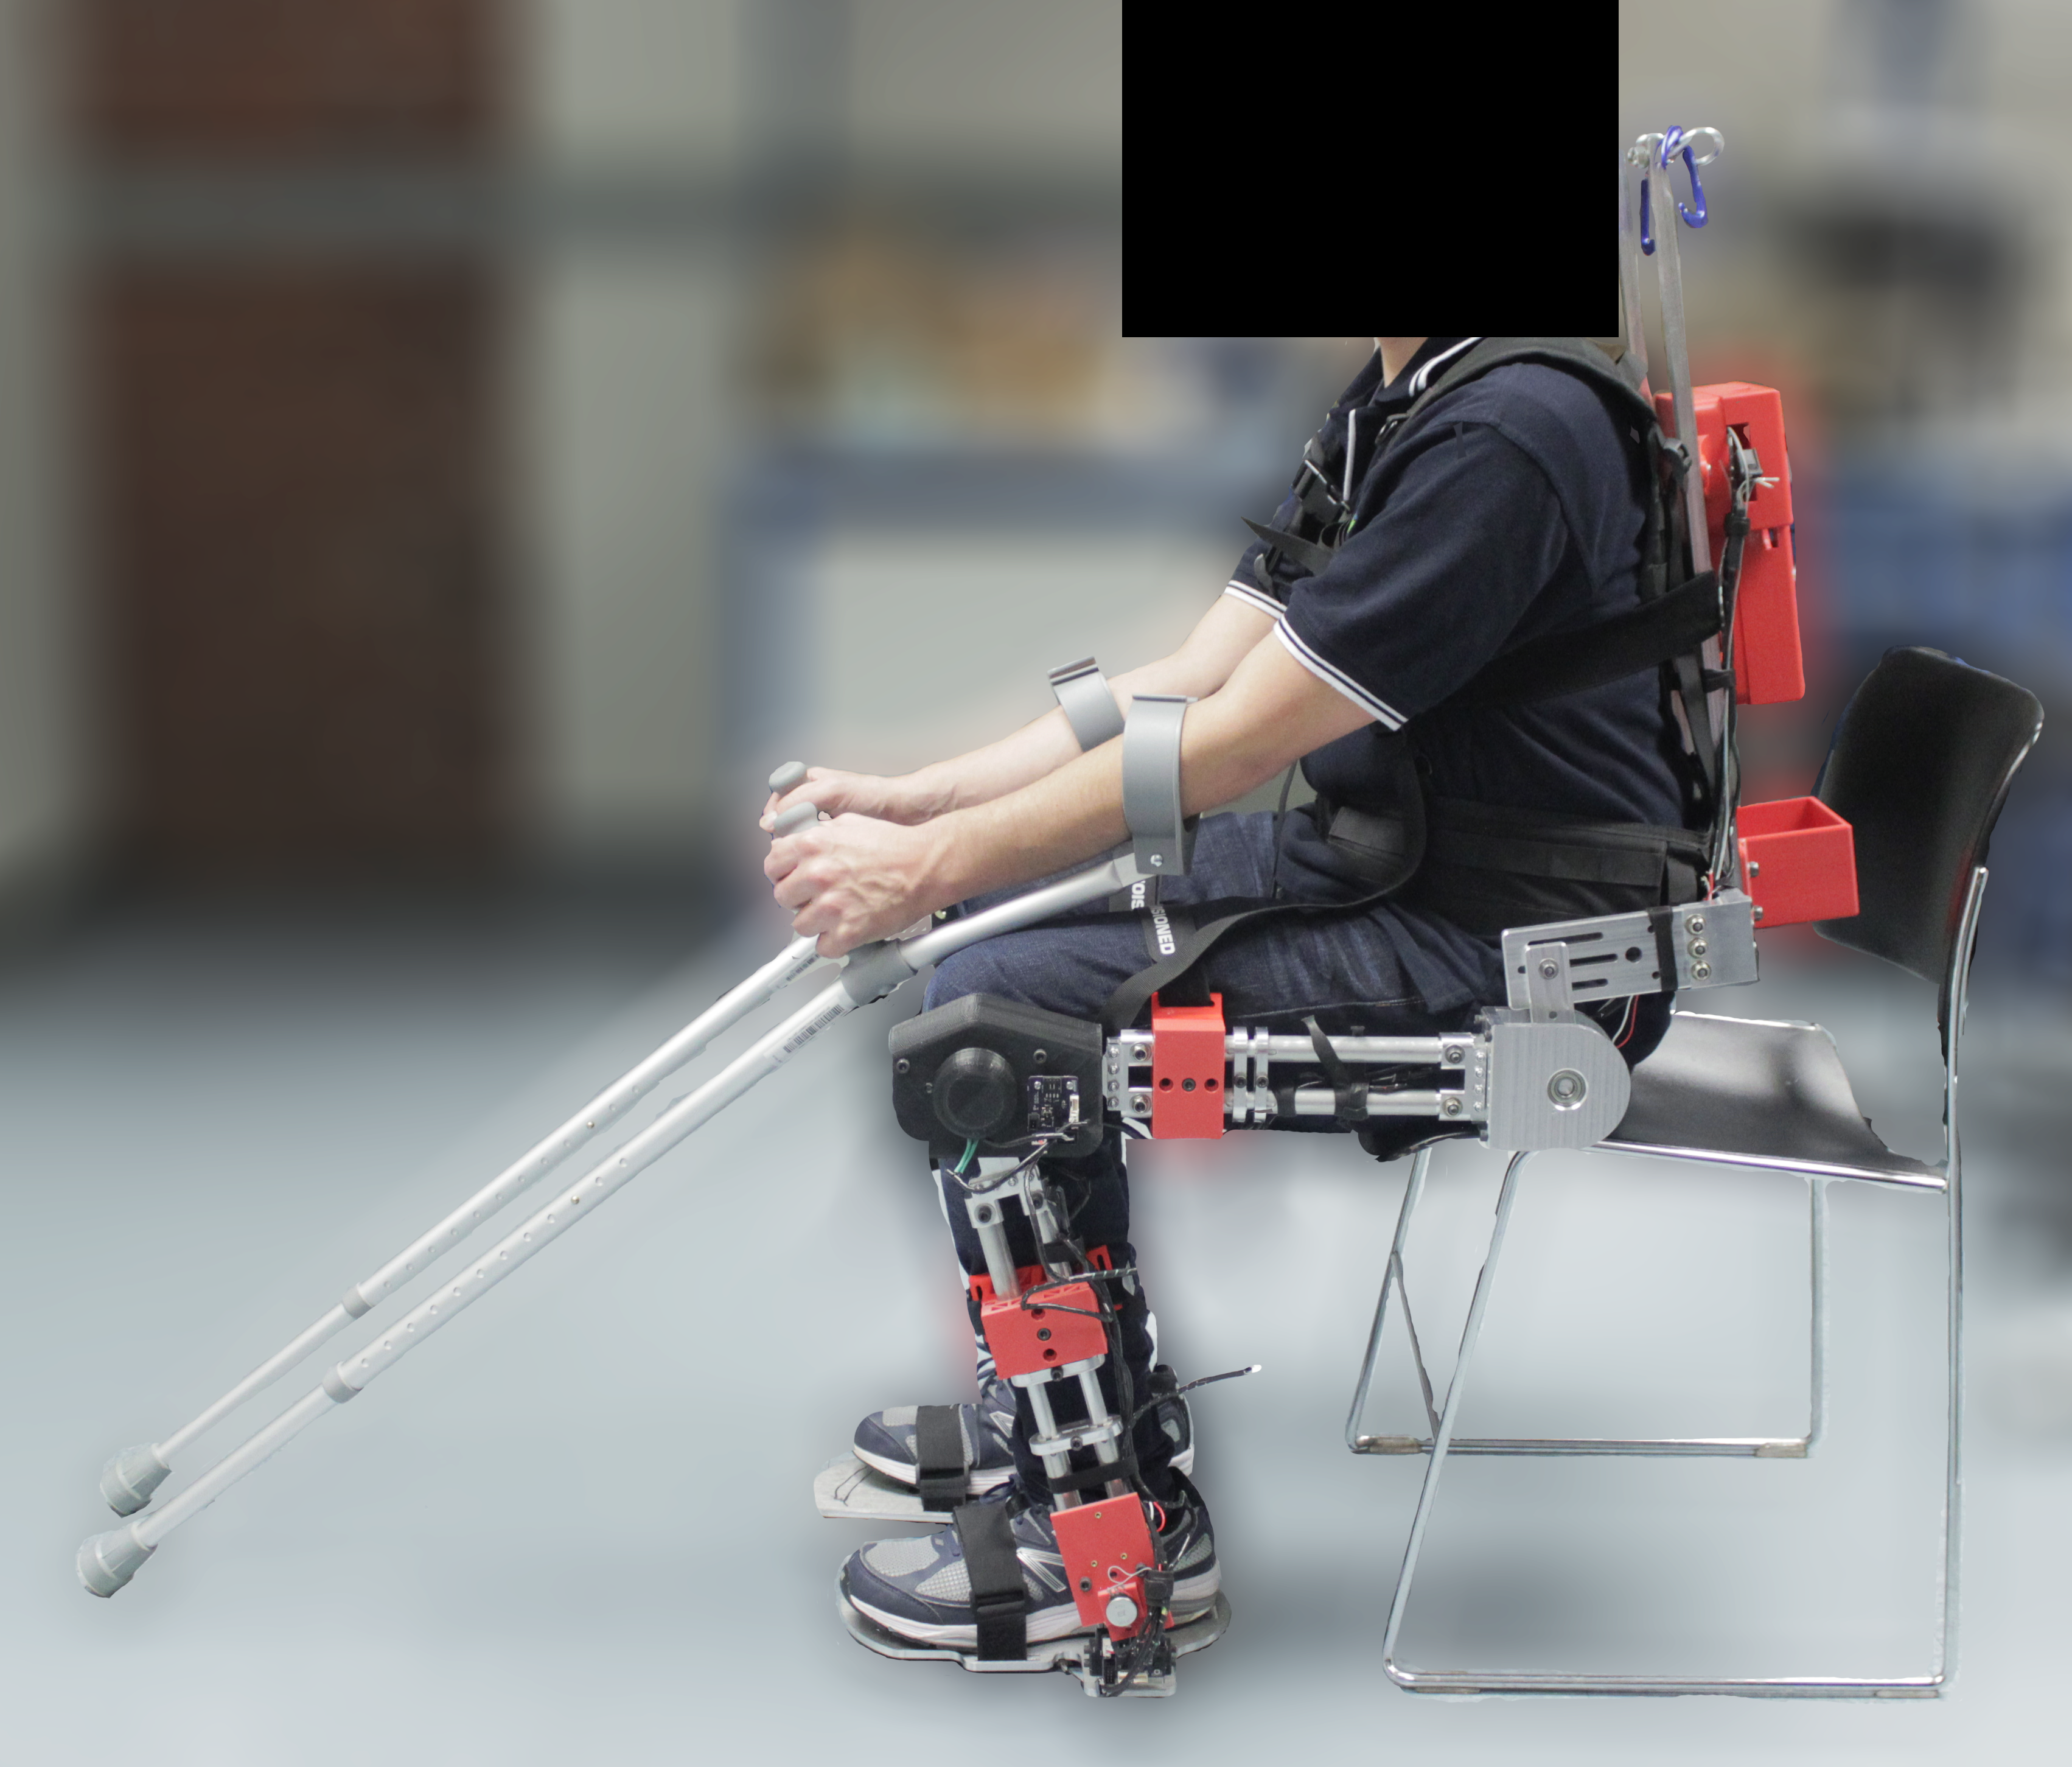
\includegraphics[scale=0.08]{images/mech_design/exo_side2.png}
    \caption{The LARRE exoskeleton being worn}
    \label{fig:LARRE}
\end{figure}


The dynamic properties of LARRE are essential for building the controller. The dynamics of LARRE were found using SolidWorks. The properties account for the material properties of the components as well as the geometry. \autoref{tab:LARREMASS} summarizes the dynamic properties of LARRE. The exoskeleton has defined joint limits to allow for biological motion, summarized in \autoref{tab:jointlimits}.

\begin{table}[h!]
    \centering
    \begin{tabular}{|c c c c c|}  
         \hline 
          \multicolumn{5}{|c|}{Exoskeleton Segment Parameters} \\
         \hline
         Link & Mass (kg) & $CoM_x$ & $CoM_y$ & $CoM_z$ \\
         \hline \hline
         Hip & 2.3677 & 0.000011338 & 0.093937 &  -0.12619 \\
         Thigh & 2.1138 & 0.0034745   & 0.097979 &  0.1712 \\
         Shank & 1.2804  &   0.002761 & 0.097563   & 0.15581\\
         Foot & 0.85523 & 0.14092 & 0.2267 &  -0.31138  \\
         \hline
    \end{tabular}    
    \caption[Dynamic Properties of the LARRE]{Mass Properties of the LARRE}
    \label{tab:LARREMASS}
\end{table}


\begin{table}[h!]
\begin{centering}
    \begin{tabular}{ |p{1cm} p{2cm} p{2cm} |  }
        \hline 
        \multicolumn{3}{|c|}{LARRE Joints Limits} \\
        \hline 
        Joint & Flexion & Extension \\
        \hline \hline
        Hip   & $-60^{\circ}$   & $30^{\circ}$  \\
        Knee &   $-110^{\circ}$  & $0$   \\
        Ankle & $-20^{\circ}$ & $20^{\circ}$  \\
        \hline
    \end{tabular}
    \caption[LARRE Joint Limits]{Joint limits}    \centering
    \label{tab:jointlimits}
\end{centering}
\end{table}


% \begin{table}[h!]
% \begin{centering}
%     \begin{tabular}{ |p{1cm} p{2cm} p{2cm} p{2cm}|  }
%         \hline 
%         \multicolumn{4}{|c|}{LARRE Joints Limits} \\
%         \hline 
%         Joint & Flexion & Extension & Torque \\
%         \hline \hline
%         Hip   & $-60^{\circ}$   & $30^{\circ}$ &  60N \\
%         Knee &   $-110^{\circ}$  & $0$  & 50N \\
%         Ankle & $-20^{\circ}$ & $20^{\circ}$ &  - \\
%         \hline
%     \end{tabular}
%     \caption[LARRE Joint Limits]{Joint limits}    \centering
%     \label{tab:biomech}
% \end{centering}
% \end{table}